\clearpage
\section{Glossy Analysis}
\subsection{Linearly connected network}
In a linear connected network, assuming every nodes are connected linearly with two neighbors.
Namely, only two nodes in the RF range of single transmission except the terminal nodes.

\begin{figure}[h]
\centering
	
\includegraphics[width=0.6\columnwidth]{glossy_linear_topology}
\end{figure}

With Glossy protocol, the number of transmission $N$ is a parameter which limits the maximum
number of transmission of each node. Assuming the packet length in time $T_p$, TXRX turnaround 
time $T_t$ and the number of hops $K$.
In the steady state, every nodes in the network wake up in the same time. Assuming all nodes
wake up at time $t = 0$ and the {\bf Initiator (I)} starts transmission after time delay 
$T_\gamma$. Figure~\ref{fig:glossy_linear_timing} is the example with I = {\bf n\subscript{1}}
and $N = 3$.

\begin{figure}[h]
\centering
	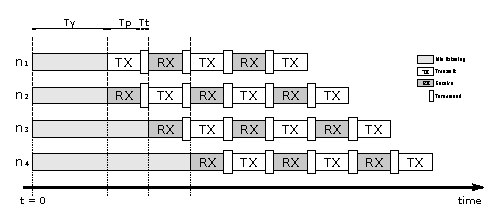
\includegraphics[width=0.9\columnwidth]{glossy_linear_timing}
	\caption{Timing diagram of a simple glossy flooding with N = 3}
	\label{fig:glossy_linear_timing}
\end{figure}

From figure~\ref{fig:glossy_linear_timing}, we can infer the radio on time for each node
in a linear connected network. Note that the following analysis is base on the assumption
that {\bf every transmission is success}, which is likely hold if no interference present.

The radio on time of initiator I is the shortest. It has to transmit $N$ times. Between $N$
transmissions, there are $N-1$ receiving slot. Therefore, sum up the total number of transmission
and receiving. We can find $2N-1$ packet length $T_p$ and $2N-2$ turnaround time $T_t$.
We can write the radio on time of Initiator $T_I$ as following:
\begin{equation}
	T_I = T_\gamma + (2N-1)T_P + (2N-2)T_t
\end{equation}
From the figure~\ref{fig:glossy_linear_timing}, we can infer that the radio on time of the node 
which is 1 hop distance from the initiator $T_{D=1}$ is $T_p + T_t$ longer than $T_I$. Since 
the node has the exactly the same pattern once it starts transmission. The time between the radio on
and starts transmitting is $T_p + T_t$.
\begin{equation}
	T_{D=1} = T_I + T_p + T_t
\end{equation}
Expand the radio on time for any nodes which is $i$ hops away from initiator $T_{D=i}$
\begin{equation}
	T_{D=i} = T_I + i\times(T_p + T_t)
\end{equation}

We define a {\bf Total Radio On Time (TROT)} as the {\bf sum of radio on time in the network}. Since
Glossy uses flooding to send packet through the entire network, the TROT of a linearly connected
network is not a constant. However, it's correlated with the {\bf position of initiator in the
network}. The intuition view is that the nodes far from initiator would have longer on time. Therefore,
the TROT is minimum if the initiator is located in the middle of the linearly connected network.
We define another term {\bf Total Distance (TD)} as the {\bf sum of distance between all nodes in the network
and initiator I}. We can correlate the TROT to TD. To calculate the TROT, we can simply
calculate the TD.
\begin{equation}
	TROT = TD\times(T_p + T_t) + K\times T_I
	\label{eq:TROT_TD}
\end{equation}
For example, if the initiator I is located in the edge of the network ($n_1$ or $n_K$), the TD 
is following:
\begin{equation}
	TD_1 = \displaystyle\sum\limits_{i=0}^{K-1} i = \tfrac{K(K-1)}{2}
\end{equation}
Similarly, if the initiator I is located in 2\superscript{rd} position of the network ($n_2$ or $n_{K-1}$).
TD can be written as following:
\begin{equation}
	TD_2 = \displaystyle\sum\limits_{i=0}^{K-2} i + 1 = \tfrac{(K-1)(K-2)}{2} + 1
\end{equation}
Expand to j\superscript{th} position of the network. Where $1\le j\le K$.
\begin{align}
	TD_j = \displaystyle\sum\limits_{i=0}^{K-j} i + \displaystyle\sum\limits_{i=0}^{j-1} i &= \tfrac{(K-j+1)\times(K-j)}{2} + \tfrac{j(j-1)}{2}\\
	&=\tfrac{K(K+1)}{2} + j^2 - j\times(K+1)
\end{align}
Another assumption made here is that every nodes in the network has the same probability (uniform 
distribution) to act as initiator I. Namely, $p_{j=1} = p_{j=2} \cdots = p_{j=K-1} = p_{j=K} = 1/K$

Therefore, the average TD can be expressed as follows:
\begin{align}
	TD_{avg} 	&= \tfrac{1}{K} \displaystyle\sum\limits_{j=1}^K TD_j\\
				&= \tfrac{1}{K} \displaystyle\sum\limits_{j=1}^K \tfrac{K(K+1)}{2} + j^2 - j\times(K+1)\\
				&= \tfrac{1}{K} [\tfrac{K(K+1)}{2}\times K + \tfrac{K(K+1)(2K+1)}{6} - \tfrac{K(K+1)}{2}\times(K+1)]\\
				&= \tfrac{K(K+1)}{2} + \tfrac{(K+1)(2K+1)}{6} - \tfrac{(K+1)^2}{2}\\
				&= \tfrac{K^2-1}{3}
\end{align}
From equation~\ref{eq:TROT_TD}, the average TROT can be written as following:
\begin{align}
	TROT_{avg} 	&= TD_{avg}\times(T_p + T_t) + K\times T_I\\
				&= \tfrac{K^2-1}{3}\times(T_p + T_t) + K\times[T_\gamma + (2N-1)T_P + (2N-2)T_t]
\end{align}
The average radio on time for each node $T_{on, avg} = TROT_{avg}/K$. If $K^2\gg1$
\begin{equation}
	T_{on, avg} \approx \{\tfrac{K}{3}\times(T_p + T_t)\} + \{T_\gamma + (2N-1)T_P + (2N-2)T_t\}
	\label{eq:ton_avg}
\end{equation}
From equation~\ref{eq:ton_avg}, we can find the average radio on time in a linear connected network
is composed of two parts. The first half is only correlated to {\bf the size of the network K} and the 
second half is only correlated to {\bf the number of transmission N}. In a practical example,
$K$ = 10, $T_p$ = 0.8~ms (8 bytes data + 17 overhead~\footnote{ 4 bytes preamble, 1 byte SFD, 1 byte Length,
2 bytes FCF, 1 byte DSN, 6 bytes address (2 bytes for source/destination/PAN), 2 bytes FCS
}), $T_t$ = 192~$\mu$s + 23.5~$\mu$s (192~$\mu$s is the standard
turnaround time, 23.5~$\mu$s is SW delay implemented by Ferrai et al.~\cite{ferrari:efficient}), $N$ = 6 is 
reasonable in a linear connected network since every node has only two neighbors. If $N$ is too small, 
single transmission fails cause the packet unable to deliver to every node in the network.  $T_\gamma$ is 
affected by three factors. 
1) clock stability, 2) duty cycle period ($T$) and 3) the radio on time. Assume clock stability $= \pm$40~ppm,
$T$ = 1~s and crystal start-up time = 1~ms. We assume $T_\gamma$ = 1.5~ms in this case. Given these parameters,
the $T_{on, avg}$ in a linearly connected network is calculated as 15.84~ms.
\begin{table}[h]
\centering
	\begin{tabular}{|c|c|}
	\hline
	{\bf parameters} & {\bf value}\\ \hline
	$K$ 	& 10\\ \hline
	$T_p$ 	& 0.8~ms\\ \hline
	$T_t$	& 0.2155~ms\\ \hline
	$N$		& 6\\ \hline
	$T_\gamma$& 1.5~ms\\ \hline\hline
	$T_{on, avg}$& 15.84~ms\\ \hline
	\end{tabular}
\end{table}

\clearpage
\subsection{Grid network}
Considering a network structure that each node is {\bf on grid} and the minimum distance between
each node is 1. In addition, all the radio has its {\bf radio range = 1}. In other words, the nodes
in diagonal is out of 1 hop distance.
\begin{figure}[h]
\centering
	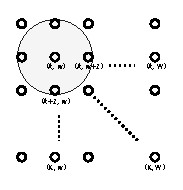
\includegraphics[width=0.4\columnwidth]{glossy_grid_topology}
	\caption{Topology of grid network. The small circles are nodes and big circle indicates the 
	1 hop radio range}
\end{figure}

From previous session, we know the average of total distance for every initiator position in a linearly 
connected network is equal to $\tfrac{K^2-1}{3}\equiv TD_0$. 
The total distance of the column which next to the one hosts the initiator I. $TD_{D=1}$ can be written
as:
\begin{equation}
 TD_{D=1} = TD_0 + K 
\end{equation}
We can calculate the total distance for the grid network with any initiator location.
For example, if the initiator is located in the left most column. $TD_{grid\ network,\ I=W_0}$ can be written as:
\begin{align}
	\nonumber
	TD_{grid\ network,\ I=W_0} 	&= TD_0 + TD_{D=1} + TD_{D=2} +\cdots TD_{D=W-2} + TD_{D=W-1}\\
						&= TD_0 + (TD_0+K) + (TD_0+2K) +\cdots (TD_0 + (W-2)K) + (TD_0 + (W-1)K)\\
						&= W\times TD_0 + K\times \displaystyle\sum\limits_{j=1}^{W-1} j
\end{align}
The average distance over entire nodes in a grid network in this case is:
\begin{equation}
	D_{avg,\ I=W_0} = \tfrac{TD_{grid\ network,\ I=W_0}}{W\times K}
\end{equation}
Similarly, the initiator could located in any column. The sum of total distance for every columns is following:
\begin{align}
	\nonumber
	TD_{total\ distance\ for\ every\ column}	&= TD_{grid\ network,\ I=W_0} + TD_{grid\ network,\ I=W_1} 
	+ \cdots TD_{grid\ network,\ I=W_W}\\ 
	&= W^2\times TD_0 + K\displaystyle\sum\limits_{j=1}^W\{\displaystyle\sum\limits_{i=0}^{W-j} i + \displaystyle\sum\limits_{i=0}^{j-1} i\}\\
	&= W^2\times TD_0 + K\times\tfrac{W(W^2-1)}{3}
\end{align}
Therefore, the averaged total distance of the grid network is:
\begin{align}
	TD_{total\ distance,\ avg}	&= TD_{total\ distance\ for\ every\ column}/W\\
	&= W\times TD_0 + \tfrac{K(W^2-1)}{3}\\
	&= W\times\tfrac{K^2-1}{3} + K\times\tfrac{W^2-1}{3}
\end{align}
The average distance for each node is:
\begin{align}
	D_{avg} &= TD_{total\ distance,\ avg}/(W\times K)\\
	&= \tfrac{K^2-1}{3W} + \tfrac{W^2-1}{3K}
\end{align}
From equation~\ref{eq:ton_avg}, we can conclude that the average on time of a node in a grid
network $T_{on,\ avg,\ grid}$ 
\begin{equation}
	T_{on,\ avg,\ grid} = {[\tfrac{K^2-1}{3W} + \tfrac{W^2-1}{3K}]\times(T_p + T_t)} + {T_\gamma + (2N-1)T_P + (2N-2)T_t}
\end{equation}

Considering the grid network has the same depth (K) and width (W) equal to 5 hops and diagonal of the
network is 8 hops. Since any node in the network has at least 2 neighbors, the number of transmission
can reduce to 3 with reliable flooding. We calculate the average on time of the node in grid network
with following parameters:
\begin{table}[h]
\centering
	\begin{tabular}{|c|c|}
	\hline
	{\bf parameters} & {\bf value}\\ \hline
	$K$ 	& 5\\ \hline
	$W$		& 5\\ \hline
	$T_p$ 	& 0.8~ms\\ \hline
	$T_t$	& 0.2155~ms\\ \hline
	$N$		& 3\\ \hline
	$T_\gamma$& 1.5~ms\\ \hline\hline
	$T_{on, avg}$& 9.6116~ms\\ \hline
	\end{tabular}
\end{table}
